%===============================================================================
% Versions
\section*{Versions}

\begin{small}

Seules les versions Vx.0 sont des documents achevés~;
les autres sont à considérer comme des brouillons.

\begin{enumerate}
  \item[V3.0 -] 2 novembre 2020~:
    \begin{itemize}
    \item Document sous licence Creative Commons
      ``Attribution-ShareAlike 4.0 International''
      \url{https://creativecommons.org/licenses/by/4.0/}.
    \end{itemize}
  \item[V2.0 -] 3 décembre 2008~:
    \begin{itemize}
      \item réorganisation,
      \item mise à jour,
      \item partie sur l'utilisation.
    \end{itemize}
  \item[V1.4 - ] 30 mai 2008~:
    \begin{itemize}
      \item ajout d'une partie sur le marquage.
    \end{itemize}
  \item[V1.3 - ] 22 novembre 2007~:
    \begin{itemize}
      \item mise à jour de la partie sur l'interprocédural.
    \end{itemize}
  \item[V1.2 - ] 07 novembre 2007~:
    \begin{itemize}
      \item mise à jour de la partie sur les dépendances de contrôle.
    \end{itemize}
  \item[V1.1 - ] 20 septembre 2007~:
    \begin{itemize}
      \item réorganisation complète,
      \item développement de la partie sur les dépendances de contrôle,
      \item discussion au sujet des boucles infinies.
    \end{itemize}
  \item[V1.0 - ] 26 juin 2007~:
    \begin{itemize}
      \item relecture et petites corrections.
    \end{itemize}
  \item[V0.2 - ] 24 mai 2007~:
    \begin{itemize}
      \item révision générale,
    \end{itemize}
  \item[V0.1 - ] 23 mars 2007~:
    \begin{itemize}
      \item création du module de calcul de PDG,
      \item extraction de la documentation du PDG du rapport sur le {\it
	slicing}.
    \end{itemize}
\end{enumerate}
\end{small}
%===============================================================================
\cleardoublepage
\tableofcontents
%===============================================================================
\cleardoublepage\chapter{Introduction}

\section{Objectif}

L'objectif initial a été de réaliser un module de \slicing
dans le cadre d'un outil généraliste d'analyse de programme (voir
\cite{ppcSlicing}).
Or, la plupart des réductions à effectuer se basent sur l'analyse des
dépendances entre les données du programme.
En effet, si l'utilisateur demande la sélection
d'une instruction \verb!return x;!, il va falloir retrouver ce qui permet de
calculer cette valeur de \verbtt{x} dans les instructions qui précèdent.\\

Il s'agit donc de calculer le \indexdef{graphe de dépendances} d'une fonction
(appelé \indexdef{PDG}~: {\it Program Dependence Graph} dans la littérature)
c'est-à-dire de représenter finement les liens de
dépendances entre les différentes instructions qui la composent.
Le résultat ce calcul est un graphe dans lequel les sommets
représentent les instructions,
éventuellement décomposées en plusieurs noeuds représentant
le calcul d'informations élémentaires.\\

Dans le cadre de l'outil de \slicing,
l'intérêt de ce calcul préalable est de pouvoir
travailler en plusieurs passes lors de l'application des
requêtes de réduction sans avoir à
refaire ce calcul qui peut être lourd (alias, dépendances partielles, etc). En
effet, même si l'on souhaite à terme calculer des réductions qui utilisent
davantage la sémantique du programme, les réductions à l'aide des dépendances
peuvent simplifier le problème.\\

Par la suite, il a été jugé intéressant de considérer ce calcul
comme un module à part entière car il peut avoir d'autres
utilités comme étudier la
propagation du flot d'information pour des analyses de sécurité, par exemple.

\section{Spécifications du PDG}\label{sec-flot}

Le PDG que l'on souhaite calculer comporte plusieurs types de dépendances~:

\subsection{Dépendances sur la valeur des données}

Les \indextxtdef{dépendances sur la valeur}{dépendance!valeur}
d'une donnée sont les plus intuitives.

\begin{exemple}
  \begin{tabular}{m{3.5cm}m{\dimexpr\linewidth-4.5cm}}
\begin{clisting}
x = a + b;
\end{clisting}
&
Ici, \verbtt{x} dépend de
\verbtt{a} et \verbtt{b} car la valeur de \verbtt{x} après cette instruction dépend
des valeurs de \verbtt{a} et \verbtt{b} avant.
\end{tabular}
\end{exemple}

La question se pose néanmoins de définir la granularité à laquelle
on s'intéresse aux données.
L'utilisation d'autres analyses et structures de données de \ppc
conduit à choisir la même précision
(pour plus de détail, voir par exemple l'analyse de valeurs de \ppc).

\subsection{Dépendances de calcul d'adresse}

Pour les affectations, la valeur qui est écrite en mémoire dépend de la partie
droite, mais le choix de l'adresse à laquelle on l'écrit peut également dépendre
de variables qui apparaissent dans la partie gauche.

\begin{exemple}
\begin{tabular}{m{3.5cm}m{\dimexpr\linewidth-4.5cm}}
\begin{clisting}
*p = x;
\end{clisting}
&
Ici, la valeur de la donnée modifiée dépend de \verbtt{x},
mais le choix de la case dans laquelle on la range dépend de \verbtt{p}.
En effet, si $p$ pointe sur $a$ ou $b$, c'est soit  \verbtt{a} soit \verbtt{b} qui
va être modifié.
\end{tabular}
\end{exemple}

On parle alors de \indextxtdef{dépendances sur l'adresse}{dépendance!adresse}.

\subsection{Dépendances de contrôle}

Lorsqu'une donnée peut-être modifiée par plusieurs chemins d'exécution,
elle dépend des conditions qui permettent de choisir le chemin.

\begin{exemple}
\begin{tabular}{m{3.5cm}m{\dimexpr\linewidth-4.5cm}}
\begin{clisting}
if (c)
  x = a;
L :
\end{clisting}
&
La valeur de \verbtt{x} en \verbtt{L} dépend de \verbtt{a}, mais aussi de \verbtt{c}.\\
\end{tabular}
\end{exemple}

Il s'agit d'une \indextxtdef{dépendance de contrôle}{dépendance!contrôle}.

\subsection{Dépendances sur les déclarations}

Lorsque des variables sont utilisées dans une instruction, celle-ci dépend de
leurs déclarations, car si on veut la compiler, il faut que les variables
existent.

Les déclarations des variables lues (partie droite d'une affectation) sont
considérées comme participant au calcul de la valeur.
Les déclarations des
variables utilisées pour déterminer la case affectée (partie gauche d'une
affectation) sont considérées comme des dépendances sur l'adresse.

\begin{exemple}
\begin{tabular}{m{4cm}m{\dimexpr\linewidth-5cm}}
\begin{clisting}
/* 1 */ int x;
/* 2 */ int y;
...
/* i */ x = 3;
/* j */ y = 4;
...
/* n */ x = y;
\end{clisting}
&
L'instruction (n) a une dépendance d'adresse sur la déclaration de x (1),
et des dépendances de donnée sur l'affectation de y (j)
et sa déclaration (2). Dans ce cas, on aurait pu se passer de de cette dernière
dépendance car (j) dépend déjà de (2), mais ce n'est pas forcement le cas
en présence d'alias.
\end{tabular}
\end{exemple}

\subsection{Résumé}

On voit donc qu'on distingue trois types de dépendances~:
\begin{itemize}
\item les calculs de valeurs,
\item les calculs d'adresses,
 \item le contrôle.
\end{itemize}


\section{État de l'art}\label{sec-lart}

Voyons tout d'abord ce que dit la littérature sur ce sujet
afin de voir les solutions qui peuvent répondre à notre besoin,
et les points à modifier.

\subsection{Origine}

Les graphes de dépendances ont principalement été étudiés dans le cadre du
\slicing{}, mais ils sont aussi utilisés dans les travaux sur la compilation.

\subsection{Graphes de dépendances}

\cite{Ottenstein84}, puis \cite{Ferrante87}
introduisent la notion de PDG ({\it Program Dependence Graph}).
Un tel graphe est utilisé pour représenter les différentes dépendances
entre les instructions d'un programme.
Ils l'exploitent pour calculer les instructions
qui influencent la valeur des variables en un point.\\

Cette représentation, initialement intraprocédurale, a été étendue
à l'analyse interprocédurale dans \cite{horwitz88interprocedural} où elle
porte le nom de SDG ({\it System Dependance Graph}).
Elle est maintenant, à quelques variantes près,
quasiment universellement utilisée.

\subsection{Exploitation du graphe}

Lorsque l'on utilise le graphe de dépendance pour faire du \slicing,
le calcul se résume à un problème d'accessibilité à un noeud car comme le dit
Susan Horwitz~:

\begin{definition}{slicing selon \cite{horwitz88interprocedural}}
A slice of a program with respect to program point p and variable x
consists of a set of statements of the program that might affect
the value of x at p.
\end{definition}

c'est-à-dire qu'il faut garder toutes les instructions correspondant à des
noeuds du graphe pour lesquels il existe un chemin vers le noeud représentant le
calcul de {\tt x} en {\tt p}.
Mais le problème est que ce noeud n'existe que si {\tt x} est défini
par l'instruction située en {\tt p}.

Nous verrons que cette limitation peut être levée si l'on garde
(ou recalcule) les structures de données utilisées
lors de la construction du graphe.\\

Le traitement des appels de fonction est souvent compliqué par le fait qu'il
est également ramené à un problème d'accessibilité dans un graphe qui,
cette fois, représente toute l'application. Or, dans un tel graphe,
si on ne prend pas de précautions supplémentaires,
on parcourt des chemins impossibles qui entrent dans une fonction
par un appel, et sortent par un autre site d'appel.
Ces chemins existent en effet dans le graphe,
mais pas dans la réalité.

Comme nous nous proposons de traiter ce problème de manière modulaire,
nous devrions échapper à une partie de ce problème.
Mais nous verrons par la suite que l'utilisation d'une analyse d'alias globale
produit néanmoins quelques effets de bord indésirables.

\subsection{Programmes non structurés}

Les premiers algorithmes utilisés fonctionnent
correctement sur des programmes structurés,
mais produisent des résultats erronés en présence de \verbtt{goto}.

Le problème vient du fait que ces instructions ne modifient pas de données~:
il n'y a donc pas de dépendance de donnée~; et il n'y a pas
de dépendance de contrôle non plus car dans le CFG,
une seule branche sort du noeud pour aller vers le point de branchement.

Plusieurs personnes (\cite{Choi94},  \cite{agrawal94slicing},
\cite{harman98new},  \cite{kumar02better} entre autres)
se sont donc intéressées
aux sauts (\verbtt{goto}) qui brisaient la structure du programme.
Ce point, qui nous intéresse tout particulièrement, est présenté en détail
en \S\ref{sec-cdg}.

\subsection{Pointeurs et données structurées}

De nombreux articles s'intéressent aux traitements des données structurées,
et plus encore des pointeurs. Dans le cadre de cette étude,
nous n'avons pas exploré ces recherches étant donné que
nous nous appuyons déjà sur une analyse d'alias précise.


%~~~~~~~~~~~~~~~~~~~~~~~~~~~~~~~~~~~~~~~~~~~~~~~~~~~~~~~~~~~~~~~~~~~~~~~~~~~~~~~
\section{Plan}

Les trois chapitres suivants
exposent comment est calculé notre graphe de dépendances.

Puis, nous verrons au chapitre \ref{sec-find} comment
exploiter les informations calculées et au chapitre
\ref{sec-mark} comment associer des informations aux éléments
et les propager dans le graphe.


%~~~~~~~~~~~~~~~~~~~~~~~~~~~~~~~~~~~~~~~~~~~~~~~~~~~~~~~~~~~~~~~~~~~~~~~~~~~~~~~

\cleardoublepage\chapter{Dépendances liées aux données}

Le calcul de dépendances de données et d'adresse consiste principalement
à retrouver les éléments de flot correspondant aux données utilisées dans les
expressions.
Mais comme les données peuvent être incluses les unes dans les
autres, il ne suffit pas de retrouver les éléments de flot qui calculent
exactement ces données, mais aussi ceux qui ont une intersection possible.

Par exemple, dans la séquence~:\\
  \centerline{\verbtt{d = d0; x = d.a;}}

il faut être capable de voir que \verbtt{x} dépend de \verbtt{d0}.

Autre exemple~: dans la séquence~:\\
\centerline{\verbtt{d0.a = a; d0.b = b; d = d0;}}

il faut voir que \verbtt{d} dépend éventuellement de la valeur initiale de \verbtt{d0}
(si \verbtt{d0} contient d'autres champs que \verbtt{.a} et \verbtt{.b}), mais aussi
de \verbtt{a}, et de \verbtt{b}.\\

\section{Recherche arrière}

Le premier calcul mis en {\oe}uvre procédait par recherche en arrière
des éléments de la table ayant une intersection avec les données présentes en
partie droite de l'instruction. Mais cette recherche était compliquée en cas de
dépendances partielles comme dans le second exemple ci-dessus. Cette solution a
donc été abandonnée.

\section{Propagation avant d'un état}\label{sec-propagation-etat}

La méthode finalement choisie pour calculer ces dépendances
consiste à propager en avant, par une analyse du type flot de données,
un \indexdef{état des données}
qui contient pour chaque donnée, une liste de liens vers les éléments
du graphe qui ont permis de déterminer sa valeur en ce point.

Cet état doit avoir les propriétés suivantes~:
\begin{itemize}
\item on veut pouvoir associer un nouveau noeud à une donnée
en précisant s'il faut faire l'union avec l'ensemble précédemment stocké.
Par exemple~;
\begin{itemize}
\item pour l'instruction \verbtt{x = 3;} on construit un nouvel élément
dans le PDG, et on mémorise dans l'état que \verbtt{x} est maintenant associé
à cet élément. L'ancienne association est perdue.
\item  pour l'instruction \verbtt{*p = 3;} si \verbtt{p} peut pointer sur \verbtt{x},
il faut mémoriser que  \verbtt{x} peut être défini par l'élément du PDG
correspondant, mais comme ce n'est pas sûr, il faut faire l'union avec
ce qui était précédemment stocké pour \verbtt{x}.
\end{itemize}
\item lorsque l'on demande l'ensemble associé à une donnée,
le résultat doit contenir au moins ce qu'on a stocké
(il peut contenir plus d'élément en cas de perte de précision),
\item la consultation ne doit pas modifier l'état,
\item il faut savoir faire l'union de deux états.
\end{itemize}

La structure de donnée du module \verbtt{Lmap} de \ppc correspond à ces critères,
et peut donc être utilisée pour ce calcul.\\

\section{Propagation arrière d'un état}

Une autre solution aurait pu être de propager en arrière
un état contenant les utilisations
de variables, et mettre à jour le graphe en rencontrant la définition.
Le coût de ce calcul semble être le même que le précèdent,
mais la propagation avant nous permet d'avoir, à chaque point de programme,
un état donnant la correspondance entre une donnée et les éléments du graphe,
même si cette donnée n'est pas utilisée à ce point.
Cette information nous permet par la suite de définir des critères
de \slicing moins restrictifs.

\section{Traitement de l'affectation}

Le principe de l'algorithme du traitement d'une affectation
\verbtt{lval = exp;} est donc le suivant~:

\begin{itemize}
\item recherche des données $\{d_v\}$
utilisées dans \verbtt{exp} à l'aide des résultats de l'analyse d'alias préalable,
\item calcul de {\it dpdv},
c'est-à-dire l'union des ensembles associées à ces données $d_v$ dans l'état,
\item recherche des données $\{d_a\}$
utilisées pour calculer l'adresse de {\it lval},
\item calcul de {\it dpda}
c'est-à-dire l'union des ensembles associées à ces données $d_a$ dans l'état,
\item recherche de l'élément $e$
correspondant à cette instruction dans le graphe,
      et création de cet élément s'il n'existe pas,
\item ajout des dépendances {\it dpdv} et  {\it dpda} à $e$,
\item recherche des données $\{d_x\}$
potentiellement modifiées par cette affectation,
\item calcul du nouvel état (après l'instruction)
en ajoutant dans l'ancien état un lien entre les $\{d_x\}$ et $e$.
\end{itemize}

\section{Déclarations}

Les déclarations de variable doivent être traitées séparément
des valeurs, car on peut parfois dépendre de l'adresse d'une variable
sans dépendre de ce qu'elle contient.

C'est par exemple le cas lorsque la variable apparaît à gauche
d'une affectation (\verbtt{x = 3;})
ou encore quand on n'utilise que son adresse (\verbtt{p = \&x;}).

On garde donc une table qui permet de retrouver les éléments
du graphe de dépendances qui correspondent aux déclarations.


\section{Calcul de conditions}

Les noeuds du graphe de dépendances représentant
les calculs de condition des \verbtt{if} ou \verbtt{switch}
ont des dépendances de donnée sur les données utilisées.

\section{Dépendances de donnée dans les boucles}

Pour les boucles {\it explicites}, il suffirait d'effectuer deux tours
de la boucle pour obtenir toutes les dépendances de donnée car le premier
capture les dépendances avec les données provenant d'avant la boucle,
ou interne à un tour, et le second capture les dépendances entre un tour et le
suivant.

Mais comme les boucles peuvent être introduites par la présence de sauts
quelconques,
le plus simple est dans un premier temps d'itérer jusqu'à obtenir un point fixe
sur l'état des données. Il faut noter que les noeuds ne sont créés que lors de la
première itération, les suivantes n'ajoutant que de nouvelles dépendances entre
ces noeuds. Le nombre de noeuds étant fini (de l'ordre de grandeur du nombre
d'instruction de la fonction), l'atteignabilité du point fixe est
garantie.

\section{Appels de fonction}

Le traitement des appels de fonction est présenté
dans le chapitre \ref{sec-intro-call}

\cleardoublepage\newcommand{\text}[1]{\mbox{#1}}
\newcommand{\impl}{\Rightarrow}
\newcommand{\et}{\wedge}
\newcommand{\ou}{\vee}
\newcommand{\define}{\Leftrightarrow{def}}
\newcommand{\mssi}{\Leftrightarrow}

\newcommand{\llb}{\llbracket}
\newcommand{\ch}[1]{[#1]}
\newcommand{\mch}[1]{[#1[}
\newcommand{\allch}[1]{\llb #1] }
\newcommand{\allmch}[1]{\llb #1[}

\newcommand{\n}[1]{\ensuremath{\mathfrak{#1}}}
\newcommand{\nE}{\n{E}}
\renewcommand{\P}[1]{\ensuremath{\mathit{P}(\n{#1})}}
\newcommand{\D}[2]{\ensuremath{\mathit{D}(\n{#1},\n{#2})}}
\newcommand{\Pd}[1]{\ensuremath{\mathit{Pd}(\n{#1})}}
\newcommand{\Pdi}[1]{\ensuremath{\mathit{Pd}^{\infty}(\n{#1})}}
\newcommand{\Pda}[1]{\ensuremath{\mathit{Pd}^{+}(\n{#1})}}
\newcommand{\dpdc}[1]{\ensuremath{\mathit{DpdC}(\n{#1})}}
\newcommand{\codpdc}[1]{\ensuremath{\mathit{CoDpdC}(\n{#1})}}
\renewcommand{\succ}[1]{\ensuremath{\mathit{Succ}(\n{#1})}}
\newcommand{\succl}[1]{\ensuremath{\mathit{Succ_{L}}(\n{#1})}}

\newcommand{\ssi}{si et seulement si }

\chapter{Dépendances de contrôle}\label{sec-cdg}

\section{Introduction}

Intuitivement, un noeud \n{n} du PDG a une dépendance de contrôle sur un noeud
\n{c}
si le fait d'exécuter \n{n} dépend du résultat de l'exécution de \n{c}.
Typiquement, \n{c} est un noeud qui a plusieurs successeurs, comme un {\sc if} par
exemple,
et en fonction de la branche qui est choisie, \n{n} est exécuté ou non.

Nous allons voir qu'il existe de nombreuses façons de calculer ces
dépendances de contrôle, mais que nous avons du les adapter car
elle ne correspondent pas exactement à ce que l'on souhaitait faire.
Le principal problème est que
nous nous proposons d'analyser correctement
toute fonction, même en présence de sauts quelconques, voire de boucles
infinies; ce qui, comme nous allons le voir,
pose des problèmes particuliers au niveau des dépendances de contrôle.

\section{Etat de l'art}

Commençons tout d'abord par rappeler quelques définitions
et rapporter les résultats que l'on trouve dans la littérature.

\subsection{CFG}

Le \indexdef{graphe de flot de contrôle} est un graphe orienté qui définit l'ordre
d'exécution des instructions. Un noeud \n{a} est connecté à un noeud \n{b}
si l'instruction \n{b} peut suivre immédiatement
l'instruction \n{a} dans une trace l'exécution.
On dit que \n{b} est un \indexdef{successeur} de \n{a}.
On représente l'ensemble des successeurs d'un noeud \n{a} par $\succ{a}$.
On dit aussi que \n{a} est un \indexdef{prédécesseur} de \n{b}.\\

Un noeud est considéré comme une entrée dans le CFG s'il n'a pas de prédécesseur.
Il est généralement considéré qu'il y a un unique noeud d'entrée,
et que tous les noeuds du CFG sont atteignables depuis ce point d'entrée.
Cette hypothèse semble raisonnable car on s'intéresse au CFG d'une fonction
qui a bien un seul point d'entrée, et les instructions non atteignables depuis
le point d'entrée sont du
code mort que l'on peut donc ignorer dans les analyses.\\

Un noeud est considéré comme une sortie du CFG s'il n'a pas de successeur.
Son unicité et son accessibilité sont discutées plus loin.


\subsection{Postdominateurs}

La plupart des algorithmes de calcul des dépendances de contrôle
se basent
sur un CFG dans lequel sont ajoutés deux noeuds spéciaux {\sc start} et
{\sc stop} (on notera \nE{} ce dernier),
et sur la notion de  \indexdef{postdominateur} dont une définition est
la suivante~:

\begin{definition}{postdominateur}
  Une instruction \n{a} est {\bf postdominée} par une instruction \n{b}
  (\n{b} est un {\bf postdominateur} de \n{a})
  si tous les chemins qui vont de \n{a} au noeud \nE{} contiennent \n{b}.
\end{definition}

En d'autres termes, si on passe par l'instruction \n{a},
on passe forcement par tous ses postdominateurs avant de sortir.
Ou encore,
toutes les traces partant de \n{a} et allant à \nE{} passent par \n{b}.\\


Certains auteurs définissent également
le \indextxtdef{premier postdominateur}{postdominateur!premier}
(appelé aussi \indextxtdef{postdominateur immédiat}{postdominateur!immédiat})
de la façon suivante~:

\begin{definition}{premier postdominateur}
  \n{b} est le premier postdominateur de \n{a} \ssi~:
\begin{itemize}
  \item \n{b} postdomine \n{a},
  \item et \n{b} est postdominé par tous les autres postdominateurs de \n{a}.
\end{itemize}
\n{b} est donc unique.
\end{definition}

Cela permet de construire un arbre (appelé PDT pour {\it Post-Dominator Tree})
représentant cette relation dans lequel les noeuds sont les mêmes que
ceux du CFG et le père de chaque noeud est son premier postdominateur.\\

L'ensemble des postdominateurs d'un noeud \n{a} est donné par~:
$$
\Pd{a} = \{a\} \bigcup \bigcap_{s \in \succ{a}} \Pd{s}
$$
qui traduit le fait que \n{b} postdomine \n{a} \ssi $\n{b} = \n{a}$
ou \n{b} postdomine tous les successeurs de \n{a}.
La méthode de calcul consiste à initialiser tous les ensembles à $\top$,
et à itérer jusqu'à stabilisation.
La fonction étant décroissante, la convergence est assurée.\\


La notion classique de postdominateurs suppose que le CFG ait un point unique de
sortie \nE,
et que celui-ci soit atteignable depuis tous les autres points du graphe.
Si ce n'est pas le cas, à la fin de ce calcul,
pour les \n{a} n'ayant pas de chemin vers \nE, on a~: $\Pd{a} = \top$.\\


\subsection{Dépendances de contrôle}

Intuitivement, on dit qu'une instruction \n{a} a une \indextxtdef{dépendance de
contrôle}{dépendance!contrôle} sur une instruction \n{c}
si, en fonction du choix que l'on fait en \n{c}, on passe ou non en \n{a}.
Cela suppose donc qu'il y ait un choix à faire en \n{c},
c'est-à-dire que le noeud correspondant dans le CFG
ait plusieurs successeurs.\\

Les dépendances de contrôle sont définies par \cite{Ferrante87}
de la façon suivante~:

\begin{definition}{dépendances de contrôle selon \cite{Ferrante87}}
  Pour deux noeuds \n{a} et \n{b} du CFG, \n{b} dépend de \n{a} ssi~:
\begin{itemize}
  \item il existe un chemin P de \n{a} a \n{b}
    tel que tout noeud Z de P, différent de \n{a} et de \n{b}, est postdominé
    par \n{b},
  \item et \n{a} n'est pas postdominé par \n{b}.
\end{itemize}
\end{definition}

Ce qui signifie que~:
\begin{itemize}
  \item plusieurs chemins partent de \n{a},
  \item qu'il existe un chemin qui passe par \n{b},
  \item et qu'il existe aussi un chemin qui ne passe pas par \n{b}
    (sinon, \n{a} serait postdominé par \n{b}).
\end{itemize}

Ce qui conduit à une autre
définition, équivalente à la précédente~:

\begin{definition}{dépendance de contrôle}
  Une instruction \n{b} a une {\bf dépendance de contrôle} vis à vis de \n{a} si~:
\begin{itemize}
  \item \n{b} postdomine certains successeurs de \n{a},
  \item \n{b} ne postdomine pas tous les successeurs de \n{a}.
\end{itemize}
\end{definition}

Pour calculer le CDG, l'algorithme de référence est le suivant~:

\begin{algo}{calcul du CDG selon \cite{Ferrante87}}
\begin{itemize}
\item soit ACFG le CFG (+ START et {\sc stop}) dans lequel sont ajoutés~:
  \begin{itemize}
    \item un noeud ENTRY,
    \item une arrête (ENTRY,START),
    \item une arrête (ENTRY,
      {\sc stop}),
  \end{itemize}
\item soit S l'ensemble des arrêtes (\n{a},\n{b}) de ACFG
  telles que \n{b} ne postdomine pas \n{a}, \\
  (c'est-à-dire les arrêtes partant des noeuds \n{a} qui ont plusieurs successeurs)
\item soit \n{l} le plus petit ancêtre commun à \n{a} et \n{b} dans PDT\\
  (on peut montrer que soit \n{l}=\n{a}, soit \n{l} est le père de \n{a} dans PDT)
  \begin{itemize}
    \item si \n{l} est le père de \n{a} dans PDT, tous les noeuds du PDT sur le chemin
      entre \n{l} et \n{b} (\n{b} compris, mais pas \n{l}) dépendent de \n{a},
    \item si \n{l} = \n{a}, tous les noeuds du PDT sur le chemin
      entre \n{a} et \n{b} (\n{a} et \n{b} compris) dépendent de \n{a}.
  \end{itemize}
\end{itemize}
En fait, il est plus simple de dire que  tous les noeuds du PDT sur le chemin
entre \n{b} et le père de \n{a} (\n{b} compris, mais pas le père de \n{a}) dépendent de
\n{a}.
\end{algo}

La relation de dépendance étant transitive, on peut choisir de calculer
uniquement les dépendances directes ou d'inclure les dépendances indirectes.

\begin{exemple}
\begin{tabular}{m{8cm}m{4cm}}
  Dans le CFG ci-contre, \n{b} a bien une dépendance de contrôle sur \n{a}.
  On remarque que, par contre, Z1 ou Z2 ne dépendent pas directement de \n{a},
  car ils ne postdominent pas S2. En revanche, il y a néanmoins une dépendance
  indirecte, comme on pouvait s'y attendre, car Z dépend de \n{a}, et Z1 et Z2
  dépendent de Z.
&
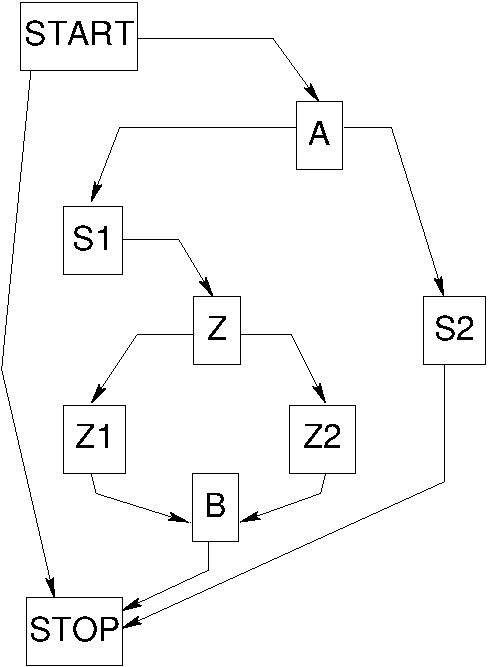
\includegraphics[width=4cm]{ctrl-dpds}
\end{tabular}
\end{exemple}

En fait, \n{a} dépend directement de c si
\n{a} est forcement atteint si on passe par l'un des successeurs de c,
mais il y a des chemins qui partent de c et qui ne passe pas pas \n{a}.

\subsection{Cas particuliers}

Ce qui a été présenté ci-dessus s'applique bien à des programmes bien
structurés, mais nécessite des adaptations si on s'intéresse~:

\begin{itemize}
  \item aux instructions qui modifie le flot de contrôle telles que les sauts,
  \item aux CFG qui contiennent des noeuds pour lesquels il n'y a pas de chemin
    vers le noeud de sortie.
\end{itemize}

Nous allons étudier plus précisément ces deux points ci-dessous.

\section{Nos définitions}

\subsection{Chemins}

Dans ce qui suit, on utilise beaucoup la notion de \indexdef{chemin}~:
un chemin est une liste de noeuds du CFG telle que si deux noeuds \n{a} et \n{b}
se suivent dans la liste, \n{b} est un successeur de \n{a}.
Nous appelons \indexdef{trace} un chemin qui se termine par un noeud
n'ayant pas de successeur, ou un chemin qui est infini.

On définit quelques notations pour désigner les chemins~:
\begin{itemize}
  \item $\ch{a, b}$  un chemin allant de \n{a} à \n{b}
  \item $\mch{a, b}$ une trace partant de \n{a} et passant par \n{b}
  \item $\mch{a, -}$ une trace partant de \n{a},
  \item $\ch{a, b, c}$ un chemin allant de \n{a} à \n{c} en passant par \n{b},
  \item $\ch{a;s, b}$
    un chemin allant de \n{a} à \n{b} en passant par $\n{s} \in \succ{a}$,
  \item $\mch{a, \neg b}$
    une trace partant de \n{a} et ne passant pas par \n{b},
\end{itemize}
et des ensembles de chemins :
\begin{itemize}
  \item $\allmch{a, -}$ toutes les traces partant de \n{a},
  \item $\allmch{a, b}$ toutes les traces partant de \n{a} et passant
    par \n{b},
  \item ...
\end{itemize}

On dit qu'un noeud appartient à un chemin, et on écrit - un peu abusivement -
$\n{x} \in \ch{a, b}$ si \n{x} apparaît au moins une fois
dans la liste qui décrit le chemin.

\subsection{Postdominateurs}

Avec les notations ci-dessus,
on peut définir \Pd{a} l'ensemble des postdominateurs de \n{a},
de la façon suivante~:
$$
  \n{b} \in \Pd{a} \define \forall t \in \allch{a, \nE}, \n{b} \in t
$$

On remarque que si on applique la définition ci-dessus à un CFG
qui contient des noeuds tels qu'il n'y a pas de chemin vers la sortie,
on a ~:
$$
\forall \n{a}, \allch{a, \nE} = \emptyset \impl \forall \n{b}, \n{b} \in \Pd{a}
$$
c'est-à-dire que l'on considère que de tels noeuds sont postdominés par tous les
autres, ce qui n'est pas très intéressant en terme de trace d'exécution~!\\

Dans ce qui suit, on note \P{a} l'ensemble des noeuds qui sont forcement
atteints quand on passe par \n{a},
et nous laisserons volontairement cette notion
un peu floue pour l'instant. Sa définition sera précisée en \S\ref{sec-pda}.

\subsection{Dépendances de contrôle} \label{sec-dpdc-if}

On définit \D{c}{s} comme
l'ensemble des noeuds qui sont forcement atteints si on passe par
\n{s}, mais pas forcement si on passe par \n{c}.
Plus formellement~:
$$
\D{c}{s} = \P{s} - \P{c}
$$
Par exemple, dans une séquence simple, si \n{c} représente un
\verbtt{if} et \n{s} la première instruction de l'une des branche, \D{c}{s}
donne les instructions de cette branche qui dépendent de la condition.\\

On définit alors $\dpdc{a}$,
l'ensemble des dépendances de contrôle de \n{a}, par~:
$$
\n{c} \in \dpdc{a} \define \n{a} \in \bigcup_{ \n{s} \in \succ{c}} \D{c}{s}
$$
Il est sans doute plus naturel de définir \codpdc{c},
l'ensemble des co-dépendances de contrôle de \n{c},
comme l'ensemble des noeuds ayant une dépendance de contrôle sur \n{c},
c'est-à-dire~:
$$
  \n{a} \in \codpdc{c} \define \n{c} \in \dpdc{a}
$$
On a alors~:
$$
\codpdc{c} = \bigcup_{ \n{s} \in \succ{c}}  \D{c}{s}
$$


On remarque que cette définition ne suppose pas que \n{c} ait plusieurs
successeurs, mais si \n{c} n'a qu'un successeur \n{s}~:
$$
\succ{c} = \{ \n{s} \} \impl
\codpdc{c} = \{\n{x} | (\exists t \in \allmch{c, -}, \n{x} \notin t)
\et (\forall t \in \allmch{s, -}, \n{x} \in t) \}
$$
or, comme \n{c} n'a qu'un successeur~:
$$
\forall t \in \allmch{c, -}, t = \mch{c; s, -}
$$
donc~:
$$
\forall t_s \in \allmch{s, -}, \n{x} \in t_s
\impl \forall t_c \in \allmch{c, -}, \n{x} \in t_c
$$
$$
\forall t_s \in \allmch{s, -}, \n{x} \in t_s
\impl \nexists t_c \in \allmch{c, -}, \n{x} \notin t_c
$$
et donc, finalement~:
$$
\succ{c} = \{ \n{s} \} \impl \codpdc{c} = \{\}
$$
Donc, un noeud n'ayant qu'un seul successeur ne peut pas être une dépendance de
contrôle. {\bf Attention}~: ceci n'est pas vrai pour les saut inconditionnels,
car ceux-ci donne lieu à un traitement spécial décrit en \S\ref{sec-goto}.


\section{Les sauts inconditionnels}\label{sec-goto}

\subsection{Présentation du problème}

Comme on l'a vu,
la définitions précédente des dépendances de contrôle conduit à
ne construire des dépendances que sur les noeuds ayant plusieurs successeurs,
c'est-à-dire ceux qui présente une forme de choix dans le CFG.
Or certaines instructions n'ayant qu'un successeur
peuvent aussi, par leur présence, modifier le flot de contrôle.
En C, c'est le cas par exemple des \verbtt{goto} explicites,
mais aussi des  \verbtt{break}, \verbtt{continue} ou \verbtt{return}.
Dans CIL, c'est aussi le cas des boucles puisqu'elles sont toutes transformées
en \verbtt{while(1)}.

Lorsque l'on souhaite utiliser le CDG pour calculer une réduction,
on aimerait
qu'il contienne également les liens nécessaires sur ces instructions
afin de déterminer si elles peuvent être supprimées,
ou si elles doivent être présentes dans le programme réduit.\\

L'exemple simple suivant, tiré de \cite{Choi94}, met en évidence ce problème~:

\begin{exemple}
\begin{tabular}{m{5cm}m{5cm}}
\begin{clisting}
1 : <entry>
2 : if (Q) goto 5;
3 : x = 4;
4 : goto 6;
5 : x = 5;
6 : y = x;
7 : <exit>
\end{clisting}
&
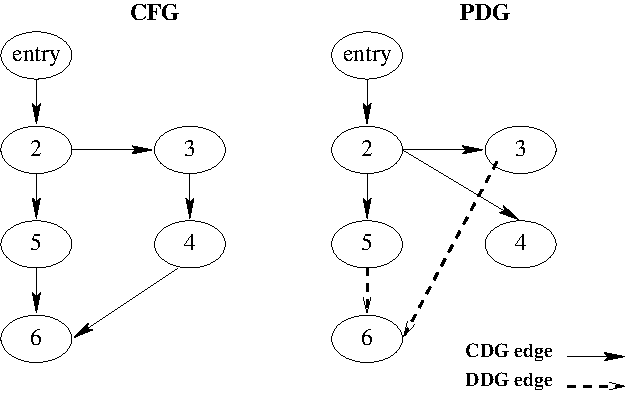
\includegraphics[width=5cm]{ex-goto}
\end{tabular}

\begin{tabular}{p{5cm} p{7cm}}
Réduction (fausse) \\
par rapport à <y,7>~:
\begin{clisting}
1 : <entry>
2 : if (Q) goto 5;
3 : x = 4;

5 : x = 5;
6 : y = x;
7 : <exit>
\end{clisting}
&
On voit que dans le graphe de dépendances (PDG), personne ne dépend de 4,
et la réduction de ce programme par rapport au noeud 6 donne le résultat
erroné ci-contre qui donne \verbtt{y=5} même lorsque $Q$ est faux.
\end{tabular}
\end{exemple}

\subsection{Etat de l'art}

La plupart des solutions proposées pour résoudre ce problème
utilisent la notion de \indexdef{successeur lexical} (sous différents noms).

\begin{definition}{successeur lexical immédiat  selon \cite{agrawal94slicing}}
A statement, S', is said to be {\bf the immediate lexical successor}
of a statement, S, in a program, if deleting S from the program
will cause the control to pass to S'
whenever it reaches the corresponding location in the new program.

If is a compound statement,
such as an If or a While statement, delleting means
delleting it allong with the statements that constitute its body.\\
\end{definition}

\cite{Choi94} présente une méthode qui ajoute un pseudo-lien dans le CFG
entre les \verbtt{goto} et leur successeur lexical immédiat,
et qui se sert de ce CFG modifié pour calculer les dépendances
de contrôle selon la méthode classique.
En fait, c'est un peu comme s'il remplaçait les \verb!goto L;!
par \verbtt{if (1) goto L;} pour mettre en évidence le chemin
qui apparaît dans le CFG si on supprime l'instruction.\\


\cite{agrawal94slicing} donne un algorithme qui permet de traiter
les \verbtt{goto} après un \slicing{} "normal".
Il s'agit, pour chaque \verbtt{goto} (G) non visible,
de déterminer si son premier postdominateur
présent dans la réduction est différent du premier successeur lexical.
Si c'est le cas, il faut rentre (G) visible ainsi que toutes ses dépendances.
Ceci donne les mêmes résultats que l'algorithme précédent,
mais il permet de ne modifier ni le CFG, ni le PDT.
Par contre, le calcul doit être fait pour chaque réduction.\\

\cite{harman98new} propose un algorithme qui donne des résultats
plus précis que les deux précédents dans certains cas.\\

Enfin, \cite{kumar02better} présente un algorithme qui prend
en compte le problème spécifique des \verbtt{switch} et donne
également de meilleurs résultats sur certains exemples.

\subsection{Discussion}\label{sec-dpdc-goto}

Dans un premier temps, l'algorithme de \cite{Choi94} semble simple à
implémenter, mais il nous oblige à calculer un nouveau CFG et le PDT
correspondant, ce que nous ne souhaitons pas faire car ces informations sont
utilisées par différents modules de l'outil.
Par ailleurs, l'algorithme de \cite{agrawal94slicing}
est à appliquer à chaque nouvelle réduction, ce qui n'est pas très intéressant
dans un environnement interactif, d'autant plus que l'on peut vouloir utiliser
les dépendances de contrôle pour autre chose que le \slicing.\\

Voyons donc plus précisément ce que l'on veut obtenir~:

\begin{monenv}{Le problème}
  \begin{tabularx}{\linewidth}{p{2cm}X}
  \begin{center}
    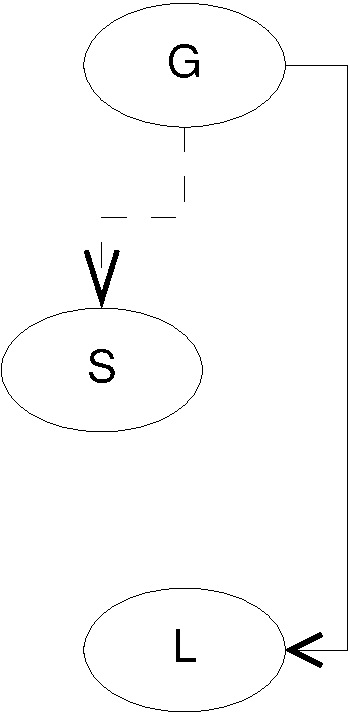
\includegraphics[width=1.5cm]{goto}
  \end{center}
&
\begin{itemize}
\item soit un programme P,
\item soit \n{g} un noeud du CFG de P correspondant à un  \verbtt{goto},
\item soit \n{l} le noeud correspondant au successeur de \n{g} (label du \verbtt{goto}),
\item soit P', le programme P dans lequel on remplace le \verbtt{goto}
par un ';' (NOP),
\item soit \n{g}' le noeud correspondant dans le CFG de P',
\item soit \n{s} le successeur lexical de \n{g}.
\end{itemize}
\bigskip
On veut qu'un noeud \n{a} ait une dépendance de contrôle sur \n{g}
\ssi \n{a} postdomine soit \n{g}, soit \n{s}, mais pas les deux.
\end{tabularx}
\end{monenv}
Examinons les différents cas~:
\begin{enumerate}
  \item si \n{s}=\n{l}, cela signifie que le \verbtt{goto} ne sert à rien,
    personne ne dépend donc de \n{g},
  \item si \n{l} postdomine \n{s}, \n{s} dépend de \n{g}, ainsi que tous les postdominateurs
    de \n{s} qui ne postdomine pas \n{l},
  \item si \n{l} ne postdomine pas \n{s},
  tous les \n{a} qui postdominent \n{s}, mais pas \n{l} ou l'inverse, dépendent de \n{g}.
\end{enumerate}

Donc, de manière générale, on peut calculer~:
$$
  \codpdc{g} = (\P{s} \cup \P{l}) - (\P{s} \cap \P{l})
$$
ce qui nous donne bien les noeuds atteints par l'une ou l'autre des branches,
mais pas par les deux.

On peut d'ailleurs montrer qu'on obtient la même chose que si on calcule \codpdc{g^*}
sur CFG$^*$ où CFG$^*$ est le CFG dans lequel le noeud \n{g} est remplacé par un
noeud \n{g^*} correspondant à une instruction
\verbtt{if (true) goto L;}\\



\section{Boucle infinie et exit}

Comme on l'a vu,
la plupart des définitions de dépendance de contrôle se basent
sur le CFG, la notion de postdominateurs, et utilisent l'hypothèse
que le CFG a un unique noeud de sortie \nE{} atteignable depuis tous les
autres points du graphe. Or, comme l'explique très bien \cite{ranganath04new},
cette hypothèse ne tient plus dans les programmes contenant
des boucles infinies ou des \verbtt{exit} (ou même des exceptions,
mais pour le langage C, nous n'avons pas le problème).
Cet article présente également avec beaucoup de détails
différents types de dépendances et des algorithmes pour les calculer,
mais il s'avère probablement trop complexe pour ce que l'on souhaite faire.\\

Le fait qu'une fonction n'atteigne pas forcement un point de sortie pose deux
problèmes différents~:
\begin{itemize}
  \item la préservation de la non-terminaison,
  \item le calcul des dépendances de contrôle pour les instructions
    n'ayant pas de chemin vers la sortie.
\end{itemize}

\subsection{Préservation de la non-terminaison}

La question qui se pose est de savoir s'il faut ajouter des dépendances de
contrôle sur les instructions qui, potentiellement, ne terminent pas.

\begin{exemple}
    \begin{tabular}{p{5.5cm}p{\dimexpr\linewidth-6.5cm}}
\begin{clisting}
while (f(x) > 0) x++;
L: y = 3;
\end{clisting}
&
Si l'on s'intéresse au calcul de {\tt y} en {\tt L}, on peut se demander si
cette instruction a une dépendance de contrôle sur la boucle,
car si dans certains cas, la boucle ne termine pas,
{\tt L} n'est pas atteint le même nombre de fois
dans le programme source P, et dans le programme P' dans lequel la boucle est
remplacée par un NOP.

\end{tabular}
\end{exemple}

Pour prendre en compte ce type de problème et permettre d'effectuer par la suite
des analyses sensibles à la non-terminaison ({\it non-terminaison sensitive}),
il faut ajouter des dépendances à toutes les instructions qui suivent
une construction qui peut ne pas terminer comme un appel de fonction,
ou une boucle dont on ne sait pas déterminer la terminaison.
Dans l'absolu, il faudrait aussi s'intéresser aux autres instructions qui ont
une terminaison anormale (\verbtt{Segmentation Fault} par exemple) mais il semble
raisonnable de considérer que ces instructions ne sont jamais présentes exprès,
et que leur absence doit être vérifiée par ailleurs.

\subsection{Postdominateurs généralisés}

\subsubsection{Définition}

En cas de boucle infinie, le CFG contient des noeuds pour lesquels
il n'existe pas de chemin vers la sortie.
Or, pour un tel noeud \n{a},
les postdominateurs tels que définis plus haut me peuvent pas être utilisé
pour déterminer les dépendances de contrôle.
En effet, on ne peut pas parler des instructions qui vont être
forcement exécutées entre \n{a} et \nE{} car il n'existe pas de telles traces.\\

La plupart des travaux existants travaillent dans ce cas sur un CFG augmenté
dans lequel le noeud \nE{} est ajouté, ainsi que des arrêtes pour le rendre
accessible. Outre le fait que certaines analyses n'aient pas besoin de cette
hypothèse, et qu'une telle modification vienne ``polluer'' le CFG,
il semble difficile (impossible ?) de ne pas ajouter
de dépendances parasites dans le cas des boucles infinies.\\

Pourtant, même si \n{a} est dans une boucle infinie,
on a intuitivement une notion de postdominateurs. On aimerait bien dire
qu'une instruction \n{b} postdomine une instruction \n{a} \ssi \n{b} appartient
à tous les chemins {\bf partant de \n{a}}, c'est-à-dire~:

\begin{definition}{postdominateurs généralisés}
$$ \n{b} \in \Pdi{a} \define \forall t \in \allmch{a, -}, \n{b} \in t $$
\end{definition}


On ne considère donc plus uniquement les chemins qui atteignent la sortie,
mais toutes les traces d'exécution possible.


\subsubsection{Méthode de calcul}


Intuitivement, si on souhaite connaître tous les noeuds qui ont b comme
postdominateurs en considérant tous les chemins,
on peut calculer les ensembles suivants~:
$$
E_b (a) = \left\{
\begin{array}{ll}
  {b} & \text{si } b = a\\
  \bigcap_{s \in \succ{a}} E_b(s) & \text{sinon.}
\end{array}\right.
$$
en partant d'ensembles initialement vides.
Ce calcul termine car il est croissant.

A la fin du calcul, on a :
$$
  \forall b, E_a (b) = \{ a \} \vee E_a (b) = \bot
$$
et $E_a (b) = \{ a \}$ veut bien dire que $a$ est dans tous les chemins entre
$b$ et $a$.\\

On peut faire ce calcul pour tous les points du CFG, et faire l'union de tous
les résultats obtenus~:
$$
\Pdi(a) = \bigcup_{b \in CFG} E_b(a)
$$
Bien sûr, ce n'est pas la manière la plus efficace de faire le calcul,
mais on voit trivialement que c'est le résultat que l'on souhaite obtenir.\\

Il suffit maintenant de trouver un calcul équivalent,
moins coûteux, mais qui termine néanmoins...

En fait, il suffit de faire directement
l'union des résultats au fur et à mesure du calcul,
mais comment prouver la terminaison~?

\subsubsection{Discussion}

On remarque que cette définition ne donne pas
les mêmes postdominateurs que précédemment
dès qu'il y a une boucle dans le CFG, même qui la sortie \nE{} est accessible
depuis tous les noeuds,
car il existe alors un chemin possible qui consiste à boucler indéfiniment.
Par conséquent, les instructions situées après la boucle ne postdomine pas les
instructions de la boucle puisqu'il existe un chemin pour lequel on y passe pas.
Cela traduit le fait que l'exécution de ces instructions dépend du fait que la
boucle termine...

Si on utilise cette définition des postdominateurs pour calculer des dépendances
de contrôle, on va donc ajouter des liens entre la boucle et tout ce qui suit.
Ces nouvelles dépendances traduisent la possible non-terminaison de la boucle,
et peuvent donc servir dans le cadre d'une analyse préservant la non-terminaison
comme on l'a vu précédemment.
Mais on ne souhaite pas nécessairement ajouter toutes ces dépendances,
car en pratique, on peut montrer par ailleurs que la plupart des boucles
d'un programme terminent.

\subsection{Postdominateurs augmentés}\label{sec-pda}

On peut essayer de faire un mélange des postdominateurs classiques et des
postdominateurs généralisés en supposant que toutes les boucles ayant une
sortie se terminent (attention : on considère pour l'instant qu'il y a un chemin
possible entre cette sortie et \nE), mais en considérant néanmoins
les traces infinies dans les cas où une boucle n'a pas de sortie.

\begin{definition}{postdominateurs augmentés}
$$
\Pda{a} = \left\{
\begin{array}{ll}
\{ b | \forall t \in \allmch{a, -}, b \in t \}
  & \text{si } \allch{a, \nE} = \{\}\\
\{ b | \forall t \in \allmch{a, \nE}, b \in t \}
  & \text{sinon.}
\end{array}\right.
$$
\end{definition}


\subsubsection{Méthode de calcul}

\newcommand{\ToRet}[1]{\ensuremath{\mathit{ToRet}(\n{#1})}}

Pour faire ce calcul, il faut être capable de distinguer les chemins qui mènent
à \nE{} des autres.
On note \ToRet{a} la propriété qui dit que \n{a} a un chemin vers \nE.

Après un calcul classique des postdominateurs (en partant de \nE),
les postdominateurs des noeuds tels que  \ToRet{a} sont établis.
Reste à calculer l'information pour les autres noeuds, c'est-à-dire ceux qui
ont les postdominateurs à $\top$.

Pour ceux-là, on fait un calcul similaire~:
$$
\Pda{x} = \{\n{x}\} \bigcup \bigcap^a_{s \in \succ{x}} \Pda{s}
$$
en redéfinissant simplement l'intersection utilisée de la façon suivante~:
$$
\Pda{a} \cap^a \Pda{b} =  \left\{
\begin{array}{ll}
  \Pda{a} \cap \Pda{b} & \text{si } \ToRet{a} = \ToRet{b}\\
  \Pda{a}              & \text{si } \ToRet{a} \et \neg\ToRet{b}\\
  \Pda{b}              & \text{si } \neg\ToRet{a} \et \ToRet{b}\\
\end{array}\right.
$$


\subsubsection{Discussion}

On remarque qu'avec cette définition, il existe des noeuds \n{a} tels que~:
$$
\succ{a} = \{\n{s1}, \n{s2}\} \et \Pda{a} \neq \Pda{s1} \cap \Pda{s2}
$$
dans le cas où on atteint la sortie à partir de l'un des successeurs, mais pas
de l'autre.

Par exemple, si on considère un noeud \n{c} correspondant à un {\sc IF}
dont l'une des branche est une boucle infinie et que l'autre permet d'atteindre
la sortie, la boucle infinie dépendra de \n{c}, alors que l'accès à la sortie
n'en dépendra pas.


\section{En résumé}

Pour calculer les dépendances de contrôle, on commence donc par calculer les
postdominateurs augmentés définis en \S\ref{sec-pda}.
Puis, pour chaque saut, on calcule ses co-dépendances de contrôle de la façon
suivante~:

\begin{itemize}
  \item pour un {\sc IF},
    on applique la définition donné en \S\ref{sec-dpdc-if},
    c'est-à-dire~:
$$
\codpdc{c} = \bigcup_{ \n{s} \in \succ{c}} \Pda{s} - \Pda{c}
$$

  \item pour un saut inconditionnel (\verbtt{goto}, \verbtt{break}, etc),
    comme mentionné en \S\ref{sec-dpdc-goto}, on calcule~:
$$
\codpdc{g} = (\Pda{s} \cup \Pda{l}) - (\Pda{s} \cap \Pda{l})
\text{  où } \left\{\begin{array}{l}
\n{s} = \succl{g} \\
\n{l} = \succ{g}
\end{array}\right.
$$
Si on considère \n{s} et \n{l} comme deux pseudo-successeurs de \n{g},
les pseudo-postdominateurs de \n{g} sont donnés par
$(\Pda{s} \cap \Pda{l})$, et on retrouve bien la formule précédente.

  \item pour les boucles, comme dans CIL, elles sont toutes infinies,
on traite la séquence \verbtt{while(1) S;}
comme si on avait \verbtt{L : S; goto L;}

\end{itemize}

\cleardoublepage\chapter{Dépendances interprocédurales}\label{sec-intro-call}

On a vu qu'un PDG est associé à une fonction.
La question se pose donc de savoir
comment calculer des dépendances interprocédurales, c'est-à-dire comment mettre
en relation les appels de fonctions et les dépendances des fonctions appelées.

Nous allons tout d'abord voir qu'un appel de fonction
est représenté par plusieurs éléments dans le PDG (\S\ref{sec-call}).
Puis, nous allons voir que pour mettre en relation des appels et les fonctions
appelées, ils faut ajouter d'autres éléments à chaque fonction
(\S\ref{sec-fct-inout}).

\section{Appels de fonction}\label{sec-call}

L'instruction contenant l'appel est représentée par plusieurs
éléments dans le graphe de dépendances
afin de pouvoir plus précisément mettre en relation les appels aux
fonctions appelées.

Les éléments créés sont les suivants~:
\begin{itemize}
\item un élément pour chaque paramètre de la fonction appelée;
  les dépendances sont crées par une simulation
  de l'affectation des arguments d'appel dans les paramètres formels,
\item un élément représentant le contrôle du point d'entrée de la fonction
  appelée (un peu comme si l'appel était dans un bloc et que ce noeud
  représentait ce bloc),
\item un élément pour chaque sortie, dépendant des entrées correspondantes.
\end{itemize}

Pour ne pas avoir à calculer les flots de données de toutes les fonctions de
l'application, il a été décidé d'utiliser les dépendances ({\it from})
calculées indépendamment par \ppc.
La liste des entrées et des sorties, ainsi que les dépendances entre les unes et
les autres sont extraites des spécifications des fonctions appelées, et non de
leur PDG\footnote{c'est peut-être un problème
si on fait de la coupure de branche, car les dépendances peuvent être réduites
par une telle spécialisation.}.
Ceci est vrai également pour les
fonctions dont le code est absent de l'application étudiée
car cela permet d'être cohérent avec les autres analyses.
Cela permettra en particulier, d'utiliser d'éventuelles propriétés
fournies par la suite par l'utilisateur.

\begin{exemple}
\begin{tabular}{m{0.35\textwidth} m{0.59\textwidth}}
\begin{verbatim}
struct {int a;
        int b; } G;

/*@ assigns \result {a},
            G.a {G, a} */
int g (int a);

int f (int x, int y) {
  G.b = x;
  x = g (x+y);
  return x + G.b;
}
\end{verbatim}
&
Ici, pour représenter l'appel à \verbtt{g} dans \verbtt{f} dans le PDG,
on va avoir~:
\begin{itemize}
  \item un élément représentant le point d'entrée dans \verbtt{g},
  \item un élément $e_1$ pour représenter \verbtt{a = x+y},
    c'est-à-dire l'affectation de l'argument de l'appel
    dans le paramètre formel de \verbtt{g},
  \item un élément $e_2$ pour calculer la valeur de retour de \verbtt{g},
    qui dépend de la valeur de $e_1$
    (utilisation de la spécification de $g$),

\item et enfin, un élément $e_3$ qui représente la seconde sortie de \verbtt{g}~:
\verbtt{G.a} qui dépend du paramètre \verbtt{a} et donc de $e_1$
    et de des éléments $\{ e_G \}$
    correspondant à
    la valeur de $G$ avant l'appel
(selon la spécification de $g$).
\end{itemize}
\end{tabular}
\end{exemple}

On note que, contrairement à ce qui était fait dans la version précédente,
on ne crée par d'élément pour l'entrée implicite $G$ de $g$ dans $f$.
Cela permet d'améliorer la précision des dépendances lorsque
l'ajout d'un tel noeud conduisait au regroupement de plusieurs données.

Ainsi, dans l'exemple précédent, on ne crée pas d'élément pour
représenter la valeur de $G$ avant l'appel, même si l'élément $e_3$ en dépend,
et on conserve donc l'information que $G.b$ ne dépend que de l'affectation
précédent l'appel.


\section{Entrées/sorties d'une fonction}\label{sec-fct-inout}

Pour relier un appel de fonction au PDG de la fonction appelée,
il faut ajouter des éléments représentant ses entrées/sorties,
c'est-à-dire~:

\begin{itemize}
  \item un élément correspondant au point de contrôle d'entrée
dans la fonction,
\item deux éléments pour chaque paramètre (cf. \S\ref{sec-decl-param}),
\item un élément pour les entrées implicites (cf. \S\ref{sec-impl-in}),
\item un élément pour la sortie de la fonction si celle-ci retourne
  quelque chose.
\end{itemize}

On note que, contrairement à ce qui était fait dans la version précédente,
on ne crée par d'élément pour les sorties implicites de la fonction.
Cela permet d'améliorer la précision des dépendances lorsque
l'ajout d'un tel noeud conduisait au regroupement de plusieurs données.

C'est par exemple le cas lorsqu'une fonction calcule $G.a$,
puis $G.a.x$ car un élément de sortie regrouperait les deux alors que
si par la suite on s'intéresse juste à $G.a.x$ à la sortie de la fonction,
le fait de ne pas avoir créé cet élément permet de retrouver l'information plus
précise.

\subsection{Entrées implicites}\label{sec-impl-in}

Au cours du calcul du PDG, on mémorise l'utilisation des données
qui ne sont pas préalablement définies.
Cela permet par la suite que créer des éléments pour ces entrées dites
implicites. On ne crée pas d'élément pour les variables locales non
initialisées, mais un message d'avertissement est émis.
Il est possible que ce soit une fausse alerte dans le cas où l'initialisation
est faite dans une branche dont la condition est forcement vrai à chaque
exécution où l'on passe par la suite par l'utilisation.

Diverses stratégies de regroupement de ces entrées peuvent être utilisées.
A ce jour, l'outil construit tous les éléments lui permettant d'avoir une
meilleure précision. C'est-à-dire que deux éléments peuvent représenter les
données qui ont une intersection.

\subsection{Déclaration des paramètres formels}\label{sec-decl-param}

En plus de l'élément représentant la valeur des paramètres,
on crée un second élément qui représente sa déclaration,
le premier dépendant du second.

Cette représentation peut permettre d'avoir une meilleure précision
dans le cas où certains calcul ne dépendent pas de la valeur du
paramètre, mais uniquement de sa déclaration.

\begin{exemple}
\begin{tabular}{m{5cm} m{\dimexpr\linewidth-6cm}}
\begin{verbatim}
int g (int a) {
  G = 2 * a;
  a = calcul_a ();
  return a;
}
int f (void) {
  int x = calcul_x ();
  return g (x);
}
\end{verbatim}
&
On voit que la valeur de retour de \verbtt{g} ne nécessite pas la valeur initiale
de \verbtt{a}, mais seulement sa déclaration. La valeur de retour de \verbtt{f}
ne dépend donc pas de l'appel à \verbtt{calcul\_x}.
\end{tabular}
\end{exemple}

Ce point n'est pas encore implémenté dans la version actuelle,
car dans des cas plus complexe, il est délicat de savoir ce qu'il faut
garder dans la fonction appelante. Le plus simple serait sans doute
de transformer le paramètre formel en une variable locale,
mais le filtrage permet à l'heure actuelle de garder ou d'effacer des
éléments existants, mais pas d'effectuer des transformations de code...

\section{Fonctions à nombre d'arguments variable}

Pour l'instant, on ne calcule pas le PDG des fonctions à nombre
d'arguments variable, c'est-à-dire que pour le reste de l'application,
tout se passe comme si on n'avait pas le code source de ces fonctions.\\

En revanche, les appels à de telles fonctions sont gérées de manière semblable à
ce qui est fait pour les autres appels, c'est-à-dire~:
\begin{itemize}
  \item création d'un noeud d'entrée pour chaque argument d'appel,
    (il y en a donc éventuellement plus que que paramètres formels dans le
    déclaration de la fonction appelée)
  \item utilisation des informations {\it from} pour créer les éventuelles
    entrées implicites, les sorties, et les liens de dépendance.
\end{itemize}

\section{Exemple}

\begin{exemple}

\lstinputlisting[language=c]{exple-call.c}
\end{exemple}

Graphe de la fonction \verbtt{f}: \\

\includegraphics[width=0.6\textwidth]{call-f}
\\

\clearpage

Graphe de la fonction \verbtt{g}: \\

\includegraphics[width=.9\textwidth]{call-g}
\\

Les graphes sont ceux qui sont effectivement produits par l'outil.

\cleardoublepage\chapter{Retrouver l'information}\label{sec-find}

Jusqu'à présent, on a vu comment calculer le graphe de dépendances.
Dans ce chapitre, nous présentons les fonctions fournies pour
trouver des éléments du PDG suivant un certain nombre de critères.
L'annexe \ref{sec-impact} rappelle certains objectifs initiaux
d'une utilisation de ces fonctions pour effectuer une analyse d'impact.\\

Par ailleurs, outre la manipulation d'ensemble d'éléments du PDG,
un système de gestion et de propagation de marques est également proposé.
Il est présenté au chapitre \ref{sec-mark}.

\section{A partir de leur clé}

Au cours du calcul, chaque élément du PDG est associé à une clé
qui correspond à l'élément de programme qu'il représente (cf. {\tt
pdgIndex.mli}).
On peut par la suite retrouver un élément à partir de cette clé
comme par exemple l'élément correspondant à une instruction simple,
à un paramètre d'entrée, à une déclaration locale, etc.

\section{A partir d'une zone mémoire}

Grâce à l'état qui est propagé lors de la construction
des dépendances de données (cf. \S\ref{sec-propagation-etat})
on peut retrouver les éléments qui participent au calcul
d'une zone mémoire à un point de programme.

Cette fonction doit également vérifier si les éléments trouvés
définissent complètement la donnée recherchée ou non,
et si ce n'est pas le cas, indiquer la zone susceptible de ne pas être
complètement définie au point considéré.

\section{A partir de propriétés}

D'autres fonctionnalités de \ppc permettent d'interpréter une propriété
du programme et d'en extraire les zones mémoire nécessaires à son évaluation.
Comme on sait par ailleurs trouver les éléments qui correspondent
a une zone mémoire en un point de programme (voir ci-dessus),
on peut ainsi trouver par exemple les éléments dont dépendent une assertion
ou tout autre propriété.

\section{En exploitant les dépendances}

Après avoir retrouver des éléments dans le graphe, on veut en général exploiter
leurs dépendances. On peut facilement retrouver les dépendances avant ou
arrière,
avec ou sans filtrage sur leur type (donnée, contrôle,...),
récursivement ou non.

\cleardoublepage\chapter{Marquage générique}\label{sec-mark}

\section{Objectif}

On souhaite pouvoir associer une information à certains éléments d'un PDG,
propager cette information dans les dépendances de ces éléments,
et calculer ce qu'il faut propager dans les autres PDG de l'application
pour avoir un traitement interprocédural cohérent. \\

Par exemple, l'information peut être un simple booléen qui indique si l'élément
correspondant est visible ou non. Pour qu'un élément soit visible, il faut que
toutes ses dépendances le soit aussi.
On voit dans cet exemple qu'on s'intéresse dans un premier temps à une
propagation arrière.\\

Comme un PDG est associé à une fonction, la propagation s'arrête aux entrées
de la fonction. Par ailleurs, les appels de fonction sont traités localement,
sans descendre dans la fonction appelée.
Pour gérer la propagation interprocédurale, les fonctions élémentaires de
marquage doivent fournir l'information à propager aussi bien dans les fonctions
appelées que dans les appelants.

\section{Marquage générique}

Le marquage pouvant être utilisé pour différents besoins,
les marques peuvent être définies par l'utilisateur.
Il lui suffit de définir comment en faire l'union.

On utilise deux types d'union~:
\begin{itemize}
  \item l'une permet de faire une simple union de deux marques,
  \item l'autre permet d'ajouter une marque à un élément de programme~:
    elle calcule donc une nouvelle marque à partir de l'ancienne,
    et de la marque à ajouter et fournit aussi la marque à propager dans les
    dépendances.
\end{itemize}

\section{Propagation arrière}

\subsection{Marquage intraprocédural}

La propagation arrière s'effectue très simplement en suivant les dépendances,
en ajoutant la marque propagée à la marque existante,
et en s'arrêtant quand la marque à propager rendue par la fonction de marquage
est $m_{\bot}$.\\

En cours de propagation, lorsque l'on traite un élément correspondant à la
sortie d'un appel de fonction, ou à une entrée de la fonction courante,
la marque à propager ainsi que l'identifiant de l'élément sont stockés.
A l'issu du marquage, on a donc~:
\begin{itemize}
  \item un ensemble de couple (entrée de la fonction, marque à propager),
  \item une liste des appels de fonction, avec pour chacun un ensemble de
    couples (sortie de l'appel, marque à propager).
\end{itemize}

C'est cette information qui permettra de faire la propagation interprocédurale.

\subsection{Propagation interprocédurale}

\subsubsection{Méthode automatique}

Le module de marquage permet de faire automatiquement
la propagation interprocédurale si on le souhaite.
Il est utilisé de cette façon dans la détection de code mort par exemple.\\

L'utilisateur peut, s'il le souhaite,
donner des fonctions de transformation des marques~:
\begin{itemize}
  \item une qui est utilisée pour transformer les marques des entrées d'une
    fonction avant la propagation dans les appelants,
  \item une autre qui est utilisée pour transformer les marques des sorties
    d'un appel de fonction avant propagation dans la fonction appelée.
\end{itemize}
Dans les cas les plus simples, ces fonctions ne font rien, et rendent
simplement la marque qui leur est passée.

\subsubsection{Méthode manuelle}

Dans certains cas, il est souhaitable de gérer cette propagation à la main.
C'est par exemple le cas dans le \slicing{} où une fonction source est associée
à plusieurs marquages différents.\\

Des fonctions aident néanmoins à retrouver les éléments à marquer dans les
autres fonctions à partir du résultat fourni par le marquage intraprocédural.
Ces fonctions traduisent les informations~:
\begin{itemize}
  \item (entrée de la fonction, marque à propager) en un ensemble d'éléments à
    marquer dans une~- ou toutes les~- fonction(s) appelante(s),
  \item (appel, \{(sortie de l'appel, marque à propager)\})
    en un ensemble d'éléments à marquer dans la fonction appelée.
\end{itemize}
Les éléments rendu sont les nouveaux points de départ de marquages
intraprocéduraux.
L'utilisateur peut, comme lors de la propagation automatique,
donner des fonctions de transformation des marques aux traductions.

\subsubsection{Données non définies}

Lorsque les points de départ marquage initial sont des éléments du PDG,
toutes les propagations s'effectueront a priori sur des éléments existant.
Mais ce n'est pas forcement le cas lorsqu'il s'agit de marquer les données
qui n'interviennent pas dans les calculs. Par exemple~:

\begin{exemple}
  \begin{verbatim}
int X1, X2;

void f (int x) { /*@ assert X1 >= 0; */ return x + 1; }

void f2 (void)  { X2 = f (2); }

void main (void) { X1 = 0; X2 = 0; f2 (); }
  \end{verbatim}

  Ici, si on s'intéresse à l'assertion de \verbtt{f}, il faut sélectionner
  \verbtt{X1} à l'entrée de \verbtt{f}, propager cette information à travers
  \verbtt{f2} pour enfin marquer l'affectation à \verbtt{X1} dans le \verbtt{main}
  alors que cette donnée n'apparaît pas dans les PDG de \verbtt{f} et \verbtt{f2}.
\end{exemple}

On voit donc que dans les informations fournies et calculées
pour gérer l'interprocédural, il peut y avoir des éléments ne correspondant
pas à des noeuds de PDG.

\subsubsection{Terminaison}

La terminaison du processus dépend de la définition des marques.
C'est donc à l'utilisateur de s'assurer que celle-ci permet la stabilisation du
marquage.

\section{Propagation avant}

La propagation avant n'est pas effectuée automatiquement à l'heure actuelle.

La propagation intraprocédurale ne pose pas de problèmes particuliers,
car elle est très semblable au calcul en arrière~: il suffit simplement de
parcourir les liens de dépendance dans l'autre sens.\\

La partie interprocédurale semble un peu plus délicate,
car il n'y a aucun point de repère dans le PDG
pour identifier les endroits à partir desquels il faut propager
(hormis le noeud correspondant au \verbtt{return}
pour la propagation vers les appelants et les arguments explicites pour
la propagation dans les appels de fonction).

Des fonctions supplémentaires sont donc fournies pour~:
\begin{itemize}
  \item trouver les noeuds d'entrées d'une fonction qui doivent être
    sélectionnés à partir des noeuds sélectionnés dans l'appelant,
  \item trouver les noeuds de sortie d'un appel de fonction
    qui doivent être
    sélectionnés à partir des noeuds sélectionnés dans la fonction appelée.
\end{itemize}

En cas d'utilisation intensive de ces fonctionnalités,
il serait sans doute intéressant de mémoriser les liens entre les
différents PDG (cela est également vrai pour la propagation interprocédurale
arrière...).\\

\cleardoublepage\chapter{Conclusion}

La version actuelle de ce greffon semble fonctionner.
Elle est utilisée par les greffons {\sc Security}, {\sc Sparecode} et
{\sc Slicing}. Ces résultats peuvent également être visualisés
graphiquement en utilisant la fonction d'exportation
au format {\tt .dot}.\\

\section{Limitations}

Les fonctions ayant un nombre d'arguments variable
ne sont pas traitées (mais les appels à de telles fonctions sont gérés).

Par ailleurs, les calculs se basant sur l'analyse de valeur,
et sur le calcul des dépendances fonctionnelles (\from)
il hérite des limitations de ces modules.

%===============================================================================
\appendix
%--------------------------------------
\cleardoublepage \chapter{Aide à l'analyse d'impact}\label{sec-impact}

Le document \cite{baudinImpact} spécifie un outil d'aide à l'analyse d'impact
après avoir analysé les besoins dans ce domaine.
L'exploitation du graphe de dépendances est présenté comme étant 
un composant important de cet outil.
Nous reprenons ici les éléments de spécification 
décrits dans le paragraphe 5.3 de ce document,
auxquels nous ajoutons quelques nouveaux critères.\\


\section{Définition d'ensembles}\label{sec-ensembles}\label{sec-defR}

\newcommand{\remitem}[1]{\begin{itemize}\item #1 \end{itemize}}
\newcommand{\warnitem}[1]{\begin{itemize}\item[$\blacktriangle$] #1
                          \end{itemize}}
\newcommand{\question}[1]{\begin{itemize}\item[{\bf ?}] #1 \end{itemize}}
\newcommand{\smilitem}[1]{\begin{itemize}\item[$\smiley$] #1 \end{itemize}}
\newcommand{\frownitem}[1]{\begin{itemize}\item[$\frownie$] #1 \end{itemize}}


Il s'agit de définir des sous-ensembles d'instructions
répondant à différents critères.

Donnons tout d'abord quelques notations :
\begin{itemize}
\item S : un ensemble d'instructions,
\item L : un point de programme,
\item V : une zone mémoire (le V se réfère à {\bf V}ariable,
mais il peut s'agir d'une donnée quelconque comme un champ de structure ou
un élément de tableau),
\end{itemize}

Les ensembles sont tous relatifs à un point de programme $L$,
et peuvent se classer en deux catégories~:
\begin{itemize}
\item ceux qui contiennent des instructions situées {\bf avant} $L$~: 
ils portent un indice 0,
\item et ceux qui contiennent des instructions situées {\bf après} $L$~:
ils portent un indice 1.\\
\end{itemize}

\begin{description}
\item[$R_0(S,L)$]  : sous-ensemble d'instructions de S depuis lesquelles 
L est accessible.
\warnitem{mais L ne postdomine pas forcement toutes les instructions de cet ensemble.} 

\item[$R_{1}(S,L)$] : sous-ensemble d'instructions de S 
qui sont (éventuellement) accessibles depuis L.

\item[$R_{L0}(S,L)$] : accessibilité à un point du code.
\remitem{il s'agit du sous-ensemble des instructions de $R_0(S,L)$
qui conditionnent le passage en L,
c'est-à-dire les instructions de branchement 
et les dépendances de ces conditions de branchement.
}

%\item[$R_{L1}(S,L)$] : ?

\item[$R_{V0}(S,L,V)$] : contenu d'une zone mémoire en un point du code.
\remitem{il s'agit du critère traditionnel de \slicing,
c'est-à-dire que cet ensemble contient les instructions de $S$ qui 
ont une influence sur la valeur de $V$ en $L$.
}

\item[$R_{V1}(S,L,V)$] : utilisation d'une zone mémoire.
\remitem{il s'agit du sous-ensemble des instructions de $R_{1}(S,L)$
influencées par la valeur qu'à la zone mémoire $V$ a en $L$.}

\item[$R_{DV0}(S,L,V)$] : définition de la valeur d'une variable à un point de
programme.
\remitem{il s'agit de l'ensemble des instructions qui {\bf définissent}
tout ou partie de la valeur de $V$ en $L$. Ces instructions 
sont donc nécessairement des affectations ou des appels de fonction.

On note que~: $R_{DV0}(S,L,V) \subseteq R_{V0}(S,L,V)$
}
\warnitem{
Il serait probablement utile d'avoir un élément spécial 
qui indique qu'il existe 
un ou plusieurs chemin menant à $L$ pour le(s)quel(s) 
$V$ n'est pas entièrement défini.
}

\item[$R_{DV1}(S,L,V)$] : modification de la valeur d'une variable.
\remitem{il s'agit de trouver les instructions $I_i$ accessibles depuis L
qui modifient la valeur de $V$,
et telles qu'il existe un chemin entre $L$ et $I_i$
le long duquel $V$ n'est pas modifiée.
Cela signifie que ces instructions sont les premières à modifier la valeur
de $V$ sur les chemins partant de $L$.}
\remitem{Il n'est pas sûr que cet ensemble soit très utile.
L'ensemble $R_{P1}(S,L,V)$ ci-dessous en sans doute plus intéressant.
}

\item[$R_{P0}(S,L,V)$] : 
portée arrière de la valeur d'une variable à un point de programme.
\remitem{il s'agit d'un sous-ensemble de $R_{L0}(S,L)$
contenant les instructions $I_i$ pour lesquelles la valeur de $V$
n'a été modifiée sur aucun chemin entre le point qui précède $I_i$ et $L$.
C'est-à-dire que la valeur de $V$ en $L$ est la même qu'avant chacune de ces
instructions, et qu'elle n'est pas modifiée entre les deux.
}

\item[$R_{P1}(S,L,V)$] : 
portée de la valeur d'une variable à un point de programme~.
\remitem{il s'agit d'un sous-ensemble de $R_{1}(S,L)$
contenant les instructions $I_i$ pour lesquelles la valeur de $V$ 
n'a été modifiée sur aucun chemin entre $L$ et le point de programme 
qui précède $I_i$.
}

\item[$R_{PV0}(S,L,V)$] : utilisation arrière d'une zone mémoire dans sa portée.
\remitem{il s'agit du sous-ensemble des instructions $R_{P0}(S,L,V)$
qui sont influencées, directement ou non, par $V$. 
}

\item[$R_{PV1}(S,L,V)$] : utilisation d'une zone mémoire dans sa portée.
\remitem{il s'agit du sous-ensemble 
         des instructions influencées, directement ou non, 
         par la valeur de $V$ en $L$
         qui sont dans la portée de cette valeur.

         On a donc : $R_{PV1}(S,L,V) = R_{V1}(S,L,V) \cap R_{P1}(S,L,V)$
        }

\end{description}

\begin{exemple1}
On montre ici différents ensembles relatifs au point $L$
et à la variable $v$~:
\end{exemple1}

\begin{center}
\begin{scriptsize}
\begin{tabular}{|l||c|c|c|c|c|c||c|c|c|c|c| }
\hline
S & $R_{0}$ & $R_{L0}$ & $R_{V0}$ & $R_{DV0}$ & $R_{P0}$ & $R_{VP0}$
            & $R_{1}$ & $R_{V1}$ & $R_{DV1}$ & $R_{P1}$ & $R_{VP1}$ \\
\hline
\verb!!                      &   &   &   &   &   &   &   &   &   &   &  \\
\verb!v = a; !               & X & X & X & X &   &   &   &   &   &   &  \\
\verb!x = b; !               & X &   & X &   &   &   &   &   &   &   &  \\
\verb!z = c; !               & X &   &   &   &   &   &   &   &   &   &  \\
\verb!if (c1>v) { !          & X & X & X &   &   &   &   &   &   &   &  \\
\verb!  z++;    !            &   &   &   &   &   &   &   &   &   &   &  \\
\verb!  }       !            &   &   &   &   &   &   &   &   &   &   &  \\
\verb!else {    !            &   &   &   &   &   &   &   &   &   &   &  \\
\verb!  if (c2) !            & X & X & X &   &   &   &   &   &   &   &  \\
\verb!    v += x; !          & X & X & X & X &   &   &   &   &   &   &  \\
\verb!    if (c3) { !        & X & X & X &   & X &   &   &   &   &   &  \\
\verb!      z += v; !        & X & X &   &   & X & X &   &   &   &   &  \\
\hline
{\tt\bf L:}
  \verb!    y = v; !         &   &   &   &   &   &   & X & X &   & X & X \\
\verb!       z++;   !        &   &   &   &   &   &   & X &   &   & X &   \\
\verb!       v++; !          &   &   &   &   &   &   & X & X &   & X & X \\
\verb!       } !             &   &   &   &   &   &   &   &   &   &   &   \\
\verb!  z += 2*y; !          &   &   &   &   &   &   & X & X &   &   &   \\
\verb!  }      !             &   &   &   &   &   &   &   &   &   &   &   \\
\verb!z += x;  !             &   &   &   &   &   &   & X & X &   &   &   \\
\verb!v = 0; !               &   &   &   &   &   &   &   &   & X &   &   \\
\verb!!                      &   &   &   &   &   &   &   &   &   &   &   \\
\hline
\end{tabular}\end{scriptsize}\end{center}
\begin{exemple2}
\end{exemple2}

La construction des ensembles ci-dessus exploite le CFG (le flot de contrôle)
et le PDG (les dépendances).\\

La construction des ensembles ci-dessous exploite en plus la sémantique du
programme car elle utilise une contrainte $C(...v_i...)$ portant
sur les valeurs des données en $L$~:

\begin{description}
\item[$R_{C0}(S,L,C(...v_i...))$] :
accessibilité contrainte à un point.
\remitem{il s'agit de déterminer l'ensemble des instructions
qui, si elles sont présentes, rendent fausse la contrainte $C$ au point $L$.
En fait, il s'agit de déplacer $C$ pour essayer de couper des branches.
La condition de branchement sera alors éventuellement
remplacée par un \verbtt{assert}.
}
\smilitem{Dans la séquence \verbtt{int x = 0; x=x-1; L:} pour laquelle
on a une contrainte $x \ge 0$, il ne s'agit pas de supprimer l'instruction
\verbtt{x=x-1;} mais bien de dire que cette branche est impossible...}

\item[$R_{C1}(S,L,C(...v_i...))$] : accessibilité contrainte depuis un point.
\remitem{il s'agit de déterminer le sous-ensemble des instructions de
$R_{1}(S,L)$ qui ne peuvent pas être atteintes si l'état en L est tel que 
$C$ est satisfaite.\\


On notera que certaines instructions n'appartenant ni à $R_{L0}$, ni à $R_{1}$
peuvent également ne pas être atteintes du fait de la contrainte.\\

}
\end{description}

\section{Exploitation du graphe pour le calcul d'ensembles}

La plupart des ensembles définis en \ref{sec-ensembles}
peuvent être calculés simplement en exploitant le flot de contrôle
et les fonction du graphe de dépendances présentées en \$\ref{sec-find}.

%-------------------------------------------------------------------------------
\cleardoublepage
\bibliographystyle{abbrvnat}
\bibliography{../slicing/design-fr/bib-slicing}
%--------------------------------------
\cleardoublepage
\printindex
%===============================================================================
